\documentclass[10pt]{article}

\input{/Users/gabesekeres/Dropbox/LaTeX_Docs/pset_preamble.tex}

\course{ECON 6100}
\pset{1}
\begin{document}
\maketitle

\begin{enumerate}
	\item Problem of shipping books. \begin{enumerate} \item In canonical form, defining $x$ as the number of books shipped from Novato to San Francisco, $y$ as the number of books shipped from Novato to Sacramento, $z$ as the number of books shipped from Lodi to San Francisco, and $w$ as the number of books shipped from Lodi to Sacramento, this problem is \begin{align*} v_P(b) = \max -(5x &+ 10y + 15z + 4w) \\ \st \qquad -x - z &\le -600 \\ \qquad -y - w &\le -400 \\ x + y &\le 700 \\ z + w &\le 800 \\ x,y,z,w &\ge 0\end{align*} In matrix form, we could represent this problem as \begin{align*} v_P(b) = \max &\;c \cdot x \\ \st \qquad Ax &\le b \\ x &\ge 0 \end{align*} where \[ A = \matrixc{-1 & 0 & -1 & 0 \\ 0 & -1 & 0 & -1 \\ 1 & 1 & 0 & 0 \\ 0 & 0 & 1 & 1}\qquad \text{ and } \qquad b = \matrixc{-600 \\ -400 \\700 \\800}\qquad \text{ and } \qquad c = \matrixc{-5 \\ -10 \\ -15 \\ -4}^T\]   \item Using the same variables as in part (a), and introducing the slack variable $\lambda \in \reals^4$, the problem in standard form is \begin{align*} v_P(b) = \max -(5x &+10y+15z+4w) + 0 \cdot \lambda \\ \st \qquad -x - z + \lambda_1 &= -600\\-y-w+\lambda_2 &= -400 \\ x + y + \lambda_3 &= 700 \\ z + w + \lambda_4 &= 800 \\ x,y,z,w &\ge 0 \\ \lambda &\ge 0 \end{align*} In matrix form, we could represent this problem as \begin{align*} v_P(b) = \max &\; c \cdot x + 0 \cdot \lambda \\ \st \qquad Ax + I_4\lambda &= b \\ x &\ge 0 \\ \lambda &\ge 0 \end{align*} where, as above, \[A = \matrixc{-1 & 0 & -1 & 0 \\ 0 & -1 & 0 & -1 \\ 1 & 1 & 0 & 0 \\ 0 & 0 & 1 & 1} \qquad \text{ and } \qquad b = \matrixc{-600 \\ -400 \\ 700 \\ 800} \qquad \text{ and } \qquad c = \matrixc{-5 \\ -10 \\ -15 \\ -4}^T\] and $I_4$ is the $4 \times 4$ identity matrix. \end{enumerate}
	\item Starting from a linear program \begin{enumerate} \item To write this problem in canonical form, we need to first deal with the free variable $y$. Define $y = y^+ - y^-$, and we can say that $y^+ ,y^- \ge 0$. Our problem in canonical form is \begin{align*}v_P(b)= \max &\; c_x x + c_y y^+ - c_y y^- \\ \st \qquad x &\le 1 \\ x,y^+,y^- &\ge 0 \end{align*} With matrices, we have that the problem is \begin{align*} \max &\; c \cdot z \\ \st \qquad Az &\le b \\ z &\ge 0 \end{align*} where \[z = \matrixc{x \\ y^+ \\ -y^-}^T \qquad c = \matrixc{c_x \\ c_y \\ c_y} \qquad  A = \matrixc{1 \\ 0 \\ 0} \qquad b = 1 \] \item Using the same variable replacement as above, and introducing the slack variable $\lambda \in \reals$, the problem in standard form is \begin{align*} v_P(b) = \max &\;c_xx+c_yy^+ - c_yy^- + 0 \cdot \lambda \\ \st \qquad x + \lambda &= 1 \\ x,y^+,y^- &\ge 0 \\ \lambda &\ge 0 \end{align*} With matrices, we have that the problem is \begin{align*} v_P(b) = \max &\; c \cdot z + 0 \cdot \lambda \\ \st \qquad Az + I^3 \lambda &= b \\ z&\ge 0 \\ \lambda &\ge 0 \end{align*} where, as above, \[ z = \matrixc{x \\ y^+ \\ -y^-}^T \qquad c = \matrixc{c_x \\ c_y \\ c_y} \qquad  A = \matrixc{1 \\ 0 \\ 0} \qquad b = 1 \]  \end{enumerate}
	\item The primal problem is \begin{align*} v_P(b) = \max &\;x_1 + 2x_2 \\ \st \qquad x_1 + x_2 &\le 4 \\ x_1 + 3x_2 &\le b \end{align*} \begin{enumerate} \item The primal problem represented in standard form, attained by introducing variables $x_1^+,x_1^-,x_2^+,x_2^+$, is \begin{align*} v_P(b) = \max &\; x_1^+ - x_1^- + 2x_2^+ - 2x_2^- \\ \st \qquad x_1^+ - x_1^- + x_2^+ - x_2^- &\le 4 \\ x_1^+ - x_1^- + 3x_2^+ - 3x_2^- &\le b \\ x_1^+,x_1^-,x_2^+,x_2^- &\ge 0 \end{align*} We have that the relevant matrices are \[c = \matrixc{1 \\ -1 \\ 2 \\ -2}^T \qquad ; \qquad b = \matrixc{4 \\ b} \qquad ; \qquad A = \matrixc{1 & -1 & 1 & -1 \\ 1 & -1 & 3 & -3}\] The dual problem is defined as \begin{align*} v_D(c) = \min&\; y \cdot b \\ \st \qquad yA &\ge c \\ y &\ge 0 \end{align*}Which becomes \begin{align*} v_D(c) = \min &\; 4y_1 + by_2 \\ \st \qquad y_1 + y_2 &\ge 1 \\ -y_1 - y_2 &\ge -1 \\ y_1 + 3y_2 &\ge 2 \\ -y_1 - 3y_2 &\ge -2 \\ y_1,y_2 &\ge 0\end{align*} \item The constraint sets for the problems are in Figure~\ref{fig:constraints} (on the next page), with the primal constraint set shaded in \textcolor{ForestGreen}{Green} and the dual constraint set in \textcolor{Purple}{Purple}. Note that the dual constraint set is a point -- it is defined precisely by the two equations $y_1+y_2 = 1$ and $y_1 + 3y_2 = 2$, the intersection of which is exactly the point $(0.5,0.5)$. The optimal points are also represented. Since the Duality Theorem holds, the same optimal value is attained in both problems -- in the primal, the value of $2.5$ is attained at the point $(5.5,-1.5)$, and in the dual the value of 2.5 is attained at the point $(0.5,0.5)$.
	
	\begin{figure}[H]
		\centering
		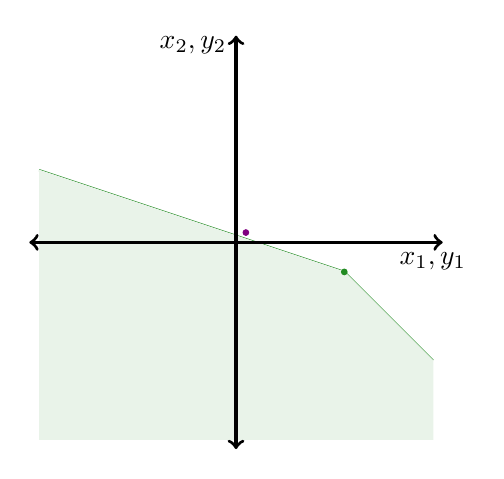
\begin{tikzpicture}[scale=0.25]
			
			\node[left] at (0,10) {$x_2,y_2$};
			\node[below] at (10,0) {$x_1,y_1$};
			
			\draw[ForestGreen,thick] (-10,3.6667)--(5.5,-1.5)--(10,-6);
			\filldraw[ForestGreen!10] (-10,3.6667)--(5.5,-1.5)--(10,-6)--(10,-10)--(-10,-10);
			\filldraw[Purple] (0.5,0.5) circle(4pt);
			\filldraw[ForestGreen] (5.5,-1.5) circle(4pt);
			
			\draw[very thick, <->] (10.5,0)--(0,0)--(0,10.5);
			\draw[very thick,<->] (-10.5,0)--(0,0)--(0,-10.5);
			
		\end{tikzpicture}
		\caption{Constraint Sets}
		\label{fig:constraints}
	\end{figure}
	
		\item The function $v_P(b)$ is, from the Vertex Theorem, always defined by the intersection of the functions $x_1 + x_2 = 4$ and $x_1 + 3x_2 = b$, where if $(x\opt_1,x\opt_2)$ is a solution to that system, $v_P(b) = x_1\opt + 2x_2\opt$. Specifically, since we have that $x_2 = 4 - x_1$, we have that $x_1 = 6 - \frac{b}{2}$, and $x_2 = \frac{b}{2} - 2$, so \[v_P(b) = 6 - \frac{b}{2} + b - 4 = 2 + \frac{b}{2}\] Thus, for $b \in [0,14]$, $\partial v_P(b) = \frac{1}{2}$. Both results are confirmed by solving the linear program for a discretization of that space, which leads to the plot in Figure~\ref{fig:obj_val}.
		
		\begin{figure}[H]
			\centering
			\includegraphics[width=10cm]{ps1_objective_value.png}
			\caption{Objective value for a range of $b$, 0 to 14 with step size 0.01.}
			\label{fig:obj_val}
		\end{figure}	
		
		The code to create this figure, as well as to solve the linear program and the dual, is:
		
		\lstinputlisting[language = Julia]{hw1_linear_program.jl}
	 \end{enumerate}
\end{enumerate}















\end{document}